\chapter{Perancangan}
\label{chap:perancangan}

Pada bab ini akan dijelaskan mengenai perancangan kelas beserta deskripsi kelas dan fungsinya, serta perancangan antarmuka.

\section{Perancangan Kelas}
\label{perancanganKelas}

Diagram kelas secara keseluruhan dapat dilihat pada gambar \ref{fig:4_class_diagram}, dimana ~terdapat ~\textit{package screensaver} (Gambar \ref{fig:4_class_diagram_screensaver}) yang didalamnya terdapat \textit{package studentportal} (Gambar \ref{fig:4_class_diagram_stupor}).
Penjelasan mengenai kelas, \textit{method}, dan atribut jsoup terdapat pada bagian \ref{sec:jsoup}.
Penjelasan mengenai kelas, \textit{method}, dan atribut JavaFX serta FXML terdapat pada bagian \ref{sec:javafx}. Penjelasan mengenai kelas, \textit{method}, dan atribut SIAModels terdapat pada bagian \ref{sec:siamodels}. Penjelasan mengenai kelas, \textit{method}, dan atribut pada \textit{package studentportal} adalah sebagai berikut:

\begin{figure}[ht]
	\centering
	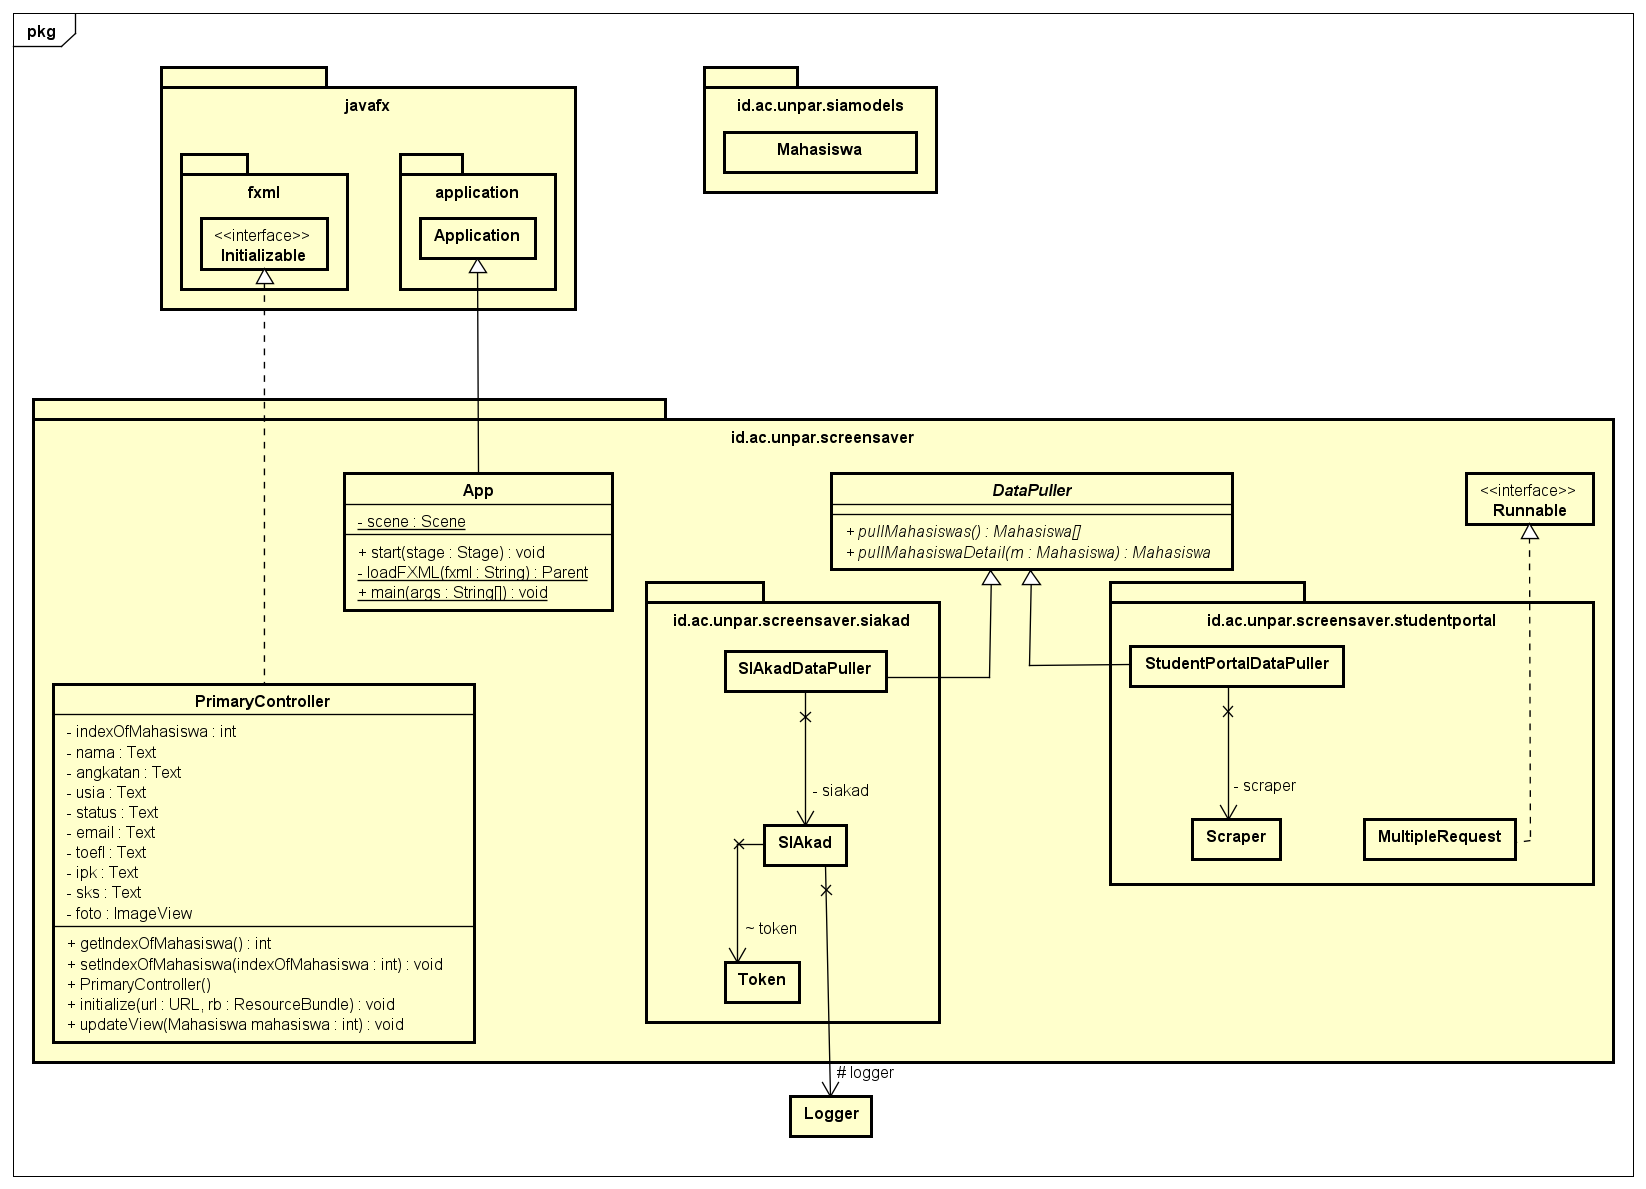
\includegraphics[angle=-90, scale=0.3]{Gambar/ClassDiagram.png}
	\caption{Diagram Kelas Keseluruhan}
	\label{fig:4_class_diagram}
\end{figure}

\begin{figure}[ht]
	\centering
	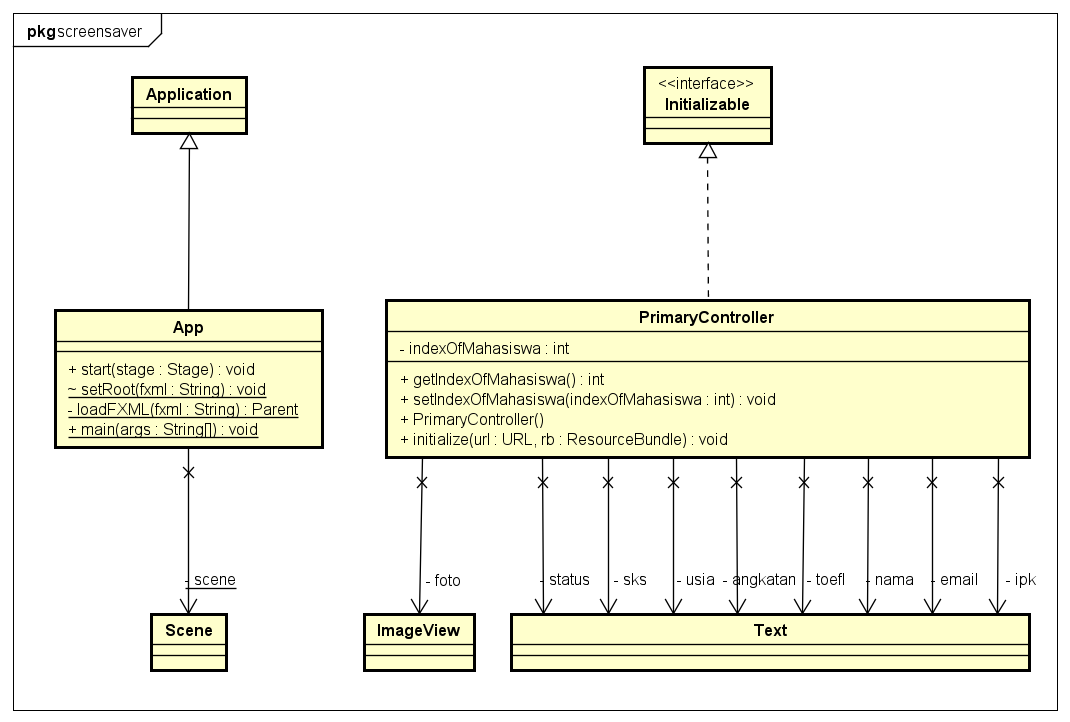
\includegraphics[scale=0.45]{Gambar/ClassDiagram_screensaver.png}
	\caption{Diagram Kelas \textit{Screensaver}}
	\label{fig:4_class_diagram_screensaver}
\end{figure}

\begin{figure}[ht]
	\centering
	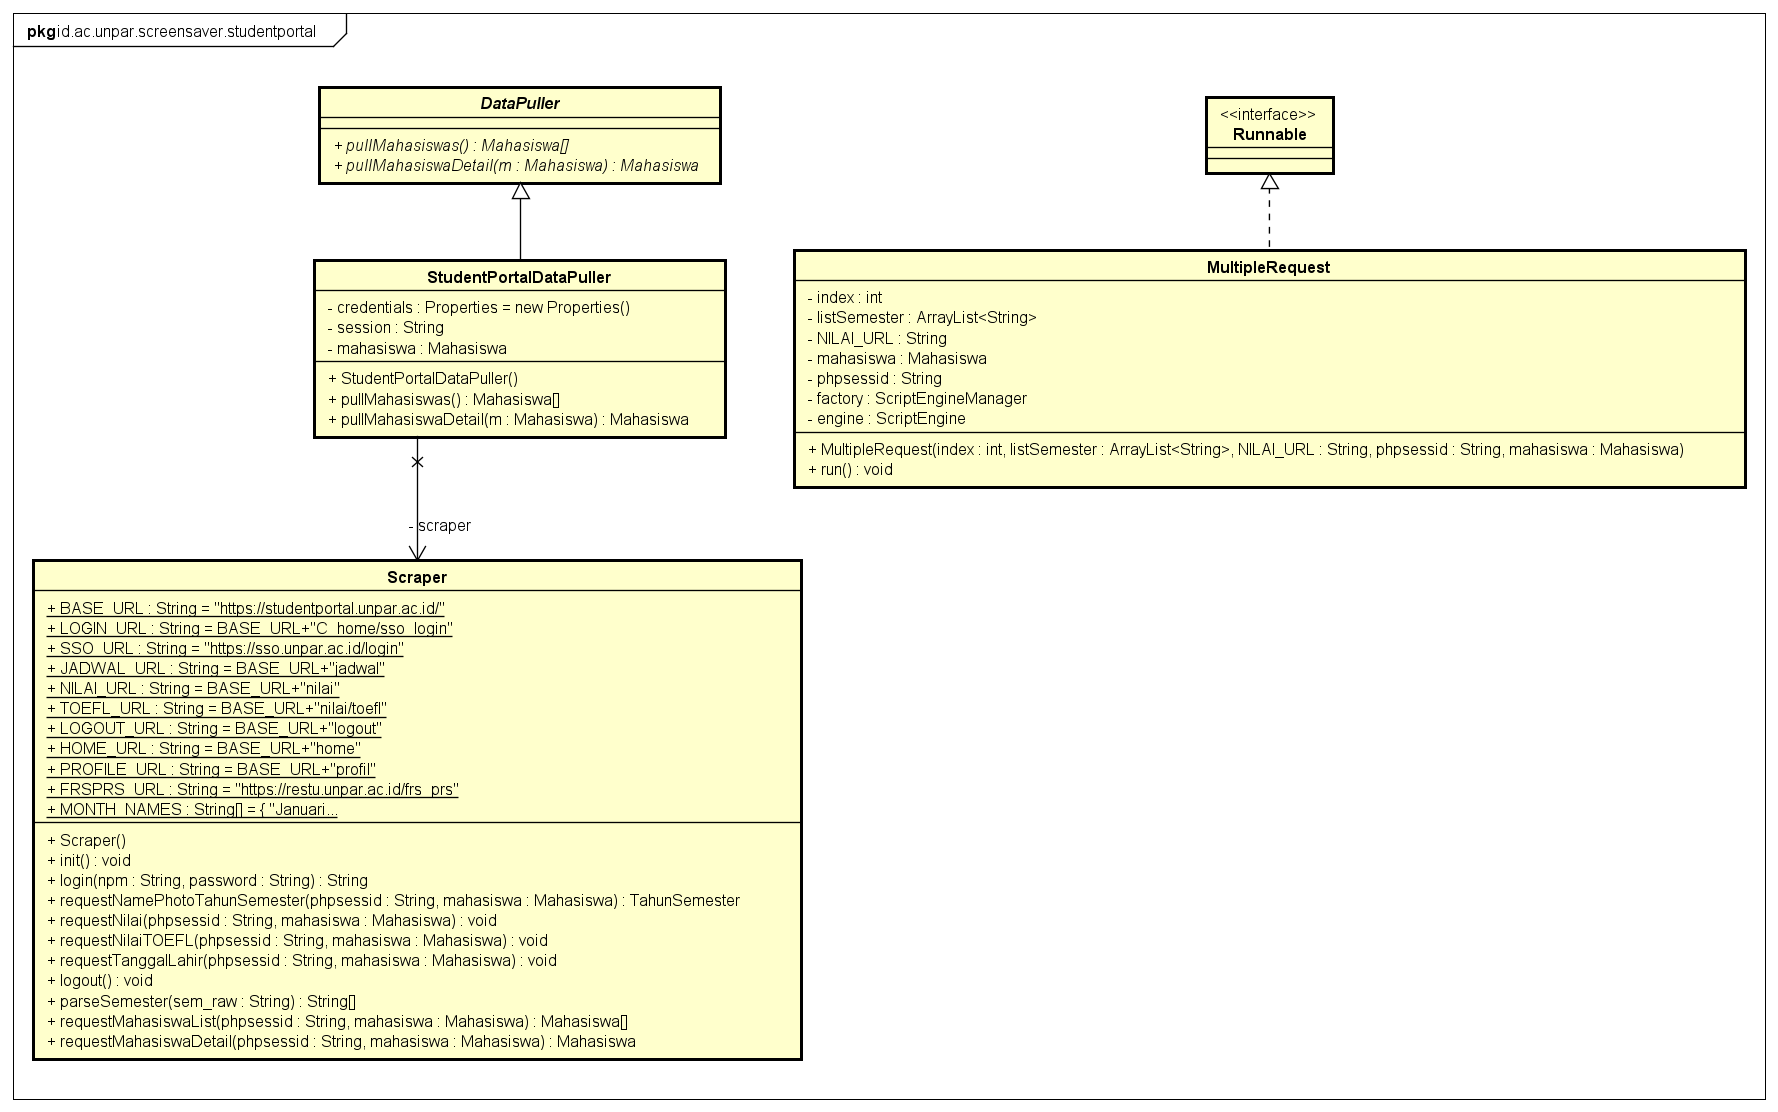
\includegraphics[scale=0.34]{Gambar/ClassDiagram_stupor.png}
	\caption{Diagram Kelas \textit{Studentportal}}
	\label{fig:4_class_diagram_stupor}
\end{figure}

\begin{enumerate}
	\item Scrapper\\
	Kelas ini memiliki fungsi untuk melakukan pengambilan data dari Portal Akademik Mahasiswa untuk kemudian diolah dan ditampilkan. Atribut yang dimiliki kelas ini adalah sebagai berikut:
	\begin{itemize}
        \item \texttt{String BASE\_URL:} menyimpan \textit{url} utama Portal Akademik Mahasiswa.
        \item \texttt{String LOGIN\_URL:} menyimpan \textit{url}  halaman \textit{login} Portal Akademik Mahasiswa.
        \item \texttt{String SSO\_URL:} menyimpan \textit{url}  halaman \textit{login} \textit{Single Sign On}(SSO) UNPAR.
        \item \texttt{String JADWAL\_URL:} menyimpan \textit{url}  halaman jadwal Portal Akademik Mahasiswa.
        \item \texttt{String NILAI\_URL:} menyimpan \textit{url}  halaman nilai Portal Akademik Mahasiswa.
        \item \texttt{String TOEFL\_URL:} menyimpan \textit{url}  halaman nilai TOEFL Portal Akademik Mahasiswa.
        \item \texttt{String LOGOUT\_URL:} menyimpan \textit{url}  untuk melakukan \textit{logout}.
        \item \texttt{String HOME\_URL:} menyimpan \textit{url}  halaman utama Portal Akademik Mahasiswa setelah melakukan \textit{login}.
        \item \texttt{String PROFILE\_URL:} menyimpan \textit{url}  halaman profil mahasiswa Portal Akademik Mahasiswa.
        \item \texttt{String FRSPRS\_URL:} menyimpan \textit{url}  halaman FRS/PRS Portal Akademik Mahasiswa.
        \item \texttt{String[] MONTH\_NAMES:} menyimpan nama-nama bulan dalam bahasa Indonesia.
	\end{itemize}
	
	\textit{Method} yang dimiliki kelas ini adalah sebagai berikut :
	\begin{itemize}
		
		\item \texttt{public Scrapper()}\\
			Berfungsi sebagai \textit{constructor} kelas \texttt{Scrapper}.
			
        \item \texttt{public void init()}\\
			Berfungsi untuk melakukan koneksi ke halaman utama Portal Akademik Mahasiswa.

		\item \texttt{public String login(String npm, String password)}\\
		    Berfungsi untuk melakukan \textit{login} ke Portal Akademik Mahasiswa.\\
		\textbf{Parameter:}
			\begin{itemize}
				\item \texttt{npm:} \textit{npm} mahasiswa yang dipakai \textit{login}.
				\item \texttt{password:} \textit{password} mahasiswa yang dipakai \textit{login}.
			\end{itemize}
		\textbf{Kembalian:} \textit{session} yang dapat digunakan untuk mengakses menu di Portal Akademik Mahasiswa.
		
	    \item \texttt{public TahunSemester requestNamePhotoTahunSemester(String phpsessid, Mahasiswa mahasiswa)}\\
		    Berfungsi untuk melakukan pengambilan nama, foto, serta semester yang sedang dijalani mahasiswa dari Portal Akademik Mahasiswa.\\
		\textbf{Parameter:}
			\begin{itemize}
				\item \texttt{phpsessid:} \textit{session} yang didapatkan dari proses \textit{login} ke Portal Akademik Mahasiswa.
				\item \texttt{mahasiswa:} objek mahasiswa yang akan ditambahkan datanya dari pengambilan data di Portal Akademik Mahasiswa.
			\end{itemize}
		\textbf{Kembalian:} semester yang sedang dijalani mahasiswa.
		
		\item \texttt{public void requestNilai(String phpsessid, Mahasiswa mahasiswa)}\\
		    Berfungsi untuk melakukan pengambilan seluruh nilai mata kuliah mahasiswa dari Portal Akademik Mahasiswa.\\
		\textbf{Parameter:}
			\begin{itemize}
				\item \texttt{phpsessid:} \textit{session} yang didapatkan dari proses \textit{login} ke Portal Akademik Mahasiswa.
				\item \texttt{mahasiswa:} objek mahasiswa yang akan ditambahkan datanya dari pengambilan data di Portal Akademik Mahasiswa.
			\end{itemize}
			
		\item \texttt{public void requestNilaiTOEFL(String phpsessid, Mahasiswa mahasiswa)}\\
	    Berfungsi untuk melakukan pengambilan seluruh riwayat nilai TOEFL mahasiswa dari Portal Akademik Mahasiswa.\\
		\textbf{Parameter:}
			\begin{itemize}
				\item \texttt{phpsessid:} \textit{session} yang didapatkan dari proses \textit{login} ke Portal Akademik Mahasiswa.
				\item \texttt{mahasiswa:} objek mahasiswa yang akan ditambahkan datanya dari pengambilan data di Portal Akademik Mahasiswa.
			\end{itemize}
			
		\item \texttt{public void requestTanggalLahir(String phpsessid, Mahasiswa mahasiswa)}\\
	    Berfungsi untuk melakukan pengambilan data tanggal lahir mahasiswa dari Portal Akademik Mahasiswa.\\
		\textbf{Parameter:}
			\begin{itemize}
				\item \texttt{phpsessid:} \textit{session} yang didapatkan dari proses \textit{login} ke Portal Akademik Mahasiswa.
				\item \texttt{mahasiswa:} objek mahasiswa yang akan ditambahkan datanya dari pengambilan data di Portal Akademik Mahasiswa.
			\end{itemize}
			
		\item \texttt{public void logout()}\\
	    Berfungsi untuk melakukan \textit{logout} dari Portal Akademik Mahasiswa.\\
		
		\item \texttt{public String[] parseSemester(String sem\_raw)}\\
	    Berfungsi untuk melakukan \textit{parsing} data semester mahasiswa dari Portal Akademik Mahasiswa agar dapat diolah lebih lanjut.\\
		\textbf{Parameter:}
			\begin{itemize}
				\item \texttt{sem\_raw:} data semester yang didapat dari Portal Akademik Mahasiswa.
			\end{itemize}
		\textbf{Kembalian:} \textit{array} yang berisi semester yang sudah dilakukan \textit{parsing}.
		
		\item \texttt{public Mahasiswa[] requestMahasiswaList(String phpsessid, Mahasiswa mahasiswa)}\\
		\label{requestMahasiswaList}
	    Berfungsi untuk mengambil seluruh mahasiswa dengan data yang diambil berupa nama, foto, semester yang sedang dijalani, dimana seluruh mahasiswa tersebut memiliki dosen wali yang sama dengan yang melakukan \textit{login} (dalam implementasi menggunakan Portal Akademik Mahasiswa, mahasiswa yang diambil adalah hanya mahasiswa yang melakukan \textit{login}).\\
		\textbf{Parameter:}
			\begin{itemize}
				\item \texttt{phpsessid:} \textit{session} yang didapatkan dari proses \textit{login} ke Portal Akademik Mahasiswa.
				\item \texttt{mahasiswa:} objek mahasiswa yang akan ditambahkan datanya dari pengambilan data di Portal Akademik Mahasiswa.
			\end{itemize}
		\textbf{Kembalian:} \textit{array} yang berisi seluruh mahasiswa yang memiliki dosen wali yang sama dengan yang melakukan \textit{login} (dalam implementasi menggunakan Portal Akademik Mahasiswa, mahasiswa yang diambil adalah hanya mahasiswa yang melakukan \textit{login}).
		
		\item \texttt{public Mahasiswa requestMahasiswaDetail(String phpsessid, Mahasiswa mahasiswa)}\\
		\label{requestMahasiswaDetail}
	    Berfungsi untuk mengambil detil lebih lanjut mengenai data mahasiswa berupa nilai TOEFL, seluruh nilai mata kuliah, tanggal lahir mahasiswa.\\
		\textbf{Parameter:}
			\begin{itemize}
				\item \texttt{phpsessid:} \textit{session} yang didapatkan dari proses \textit{login} ke Portal Akademik Mahasiswa.
				\item \texttt{mahasiswa:} objek mahasiswa yang akan ditambahkan datanya dari pengambilan data di Portal Akademik Mahasiswa.
			\end{itemize}
		\textbf{Kembalian:} objek mahasiswa yang telah ditambahkan datanya dari pengambilan data di Portal Akademik Mahasiswa.
	\end{itemize}
	
	\item{MultipleRequest}
	Kelas ini memiliki fungsi untuk melakukan koneksi ke setiap semester yang telah ditempuh mahasiswa pada halaman nilai di Portal Akademik Mahasiswa (penjelasan lebih lanjut di \ref{multipleRequest}). Atribut yang dimiliki kelas ini adalah sebagai berikut:
	\begin{itemize}
        \item \texttt{int index:} menyimpan indeks semester yang akan digunakan untuk mengakses \texttt{listSemester}.
        \item \texttt{ArrayList<String> listSemester:} menyimpan daftar semester yang telah ditempuh mahasiswa.
        \item \texttt{String NILAI\_URL:} menyimpan \textit{url} halaman nilai Portal Akademik Mahasiswa.
        \item \texttt{String phpsessid:} menyimpan \textit{session} yang dapat digunakan untuk mengakses menu di Portal Akademik Mahasiswa.
        \item \texttt{Mahasiswa mahasiswa:} menyimpan objek mahasiswa yang akan ditambahkan datanya dari pengambilan data di Portal Akademik Mahasiswa.
        \item \texttt{ScriptEngineManager factory:} untuk menjalankan \textit{javascript}.
        \item \texttt{ScriptEngine engine:} untuk menjalankan \textit{javascript}.
	\end{itemize}
	
	\textit{Method} yang dimiliki kelas ini adalah sebagai berikut :
	\begin{itemize}
		\item \texttt{public MultipleRequest(int index, ArrayList<String> listSemester, String NILAI\_URL, String phpsessid, Mahasiswa mahasiswa)}\\
		Berfungsi sebagai \textit{constructor} kelas \texttt{MultipleRequest}.
		
		\item \texttt{public void run()}\\
    	 \textit{Method} ini merupakan \textit{method} turunan dari kelas \texttt{interface Runnable}. Untuk mendapatkan data nilai dilakukan dengan cara:
    	\begin{enumerate}
    		\item Mendapatkan tahun dan semester yang ditempuh mahasiswa dari atribut \texttt{Arraylist\\<String> listSemester} diambil dari value atribut \texttt{int index}. Kemudian String dibagi menjadi tahun dan semester yang dibutuhkan.
    		\item Setelah mendapatkan tahun dan semester. Kemudian melakukan koneksi ke \textit{url} nilai berdasarkan tahun dan semester (sebagai contoh dalam gambar \ref{fig:4_nilai_script}, \textit{url} yang digunakan yaitu \url{https://studentportal.unpar.ac.id/nilai/2017/1}).
    		\item Setelah berhasil, kemudian melakukan kueri css berdasarkan script yang mengandung nilai mahasiswa (Gambar \ref{fig:4_nilai_script}). 
    		\item Selanjutnya adalah mendapatkan script yang mengandung script ``var data\_mata\_kuliah = [];'' sampai indeks dari ``var data\_angket = [];''.
    		\item Setelah mendapatkan script yang dibutuhkan, selanjutnya menjalankan script menggunakan \textit{method} milik kelas \texttt{ScriptEngine} yaitu \texttt{Object eval(String script)}.
    		\item Setelah berhasil, data yang didapatkan bertipe \texttt{ScriptObjectMirror} yang membungkus hasil eksekusi. Data nilai didapatkan dengan menggunakan \textit{method} \texttt{Object get(Object key)}.
    		\item Setelah berhasil, kemudian memasukkan data nilai ke daftar riwayat nilai mahasiswa pada atribut kelas \texttt{Mahasiswa} yaitu \texttt{List<Nilai> riwayatNilai} menggunakan method \texttt{List<Nilai> getRiwayatNilai()}. Proses ini dilakukan berulang kali sebanyak jumlah mata kuliah per semesternya.
    	\end{enumerate}
    	
    	\begin{figure}[ht]
        	\centering
        	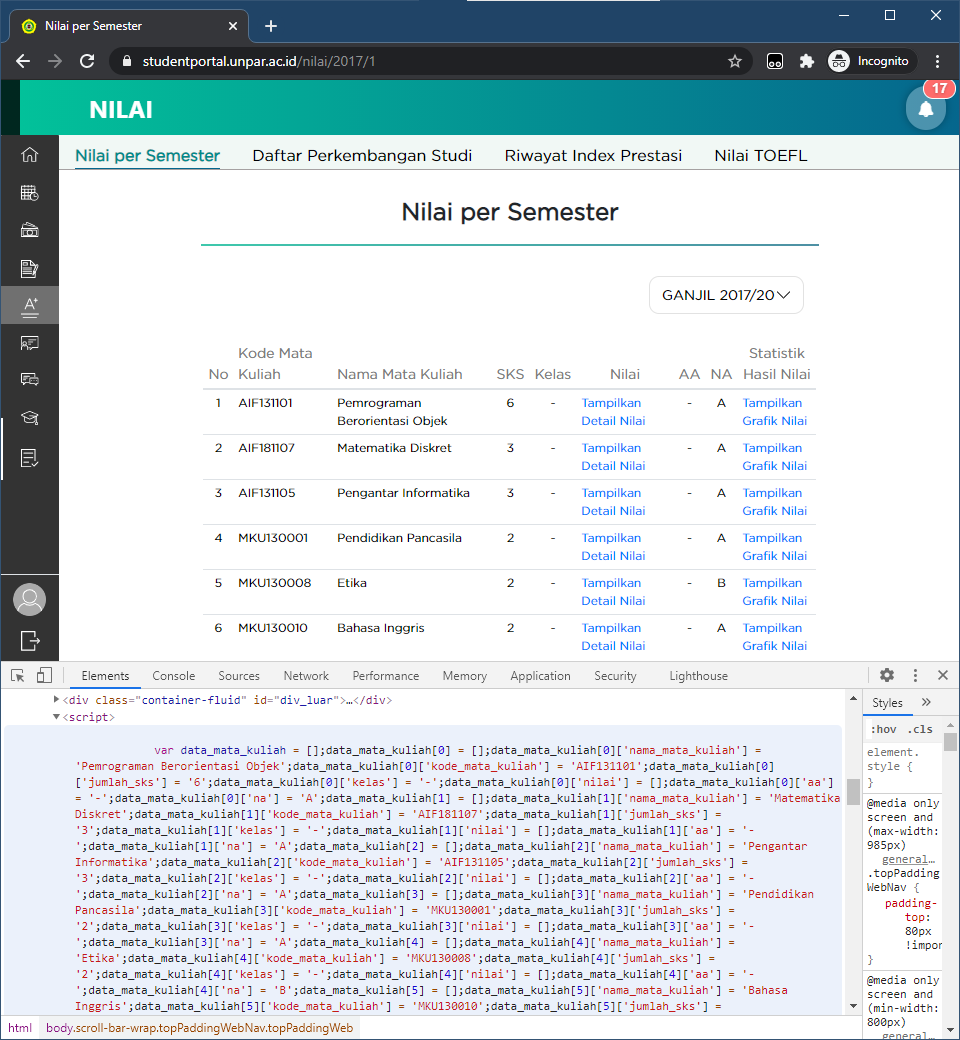
\includegraphics[scale=0.5]{Gambar/nilai_script.png}
        	\caption{\textit{Script} Data Nilai Mahasiswa Pada Halaman Nilai}
        	\label{fig:4_nilai_script}
        \end{figure}
	\end{itemize}
	
	
	\item{StudentPortalDataPuller}
	Kelas ini memiliki fungsi untuk mengambil npm dan \textit{password} mahasiswa yang disimpan dalam sebuah \textit{file}, dan kemudian memanggil \textit{method} pada kelas \texttt{Scraper}. Atribut yang dimiliki kelas ini adalah sebagai berikut:
	\begin{itemize}
        \item \texttt{Scraper scraper:} menyimpan objek \texttt{Scraper}.
        \item \texttt{Properties credentials:} mengakses \textit{file} yang berisi npm dan \textit{password} mahasiswa.
        \item \texttt{Mahasiswa mahasiswa:} menyimpan objek mahasiswa yang akan ditambahkan datanya dari pengambilan data di Portal Akademik Mahasiswa.
        \item \texttt{String session:} menyimpan \textit{session} yang dapat digunakan untuk mengakses menu di Portal Akademik Mahasiswa.
	\end{itemize}
	
	\textit{Method} yang dimiliki kelas ini adalah sebagai berikut :
	\begin{itemize}
		\item \texttt{public StudentPortalDataPuller()}\\
		Berfungsi sebagai \textit{constructor} kelas \texttt{StudentPortalDataPuller}.
		
		\item \texttt{public Mahasiswa[] pullMahasiswas()}\\
	    Berfungsi untuk memanggil \textit{method} \texttt{requestMahasiswaList} pada kelas \texttt{Scraper} (\ref{requestMahasiswaList}).\\
		\textbf{Kembalian:} \textit{array} yang berisi seluruh mahasiswa yang memiliki dosen wali yang sama dengan yang melakukan \textit{login} (dalam implementasi menggunakan Portal Akademik Mahasiswa, mahasiswa yang diambil adalah hanya mahasiswa yang melakukan \textit{login}).
		
		\item \texttt{public Mahasiswa pullMahasiswaDetail()}\\
	    Berfungsi untuk memanggil \textit{method} \texttt{requestMahasiswaDetail} pada kelas \texttt{Scraper} (\ref{requestMahasiswaDetail}).\\
		\textbf{Kembalian:} objek mahasiswa yang telah ditambahkan datanya dari pengambilan data di Portal Akademik Mahasiswa.
	\end{itemize}
\end{enumerate}

